\subsection{Anwendung}
Nachdem die Werkzeuge zur zeitlichen und kostentechnischen Schätzung theoretisch beleuchtet wurden, werden diese im Folgenden beispielhaft auf ausgewählte Komponenten des Projekts angewendet. Für die Einführung des Dokumentenmanagementsystem Alfresco wird eine TCO-Analyse sowie ein Gantt-Diagramm angefertigt. Die potentiellen Kosten des Redesigns der Hochschulwebseite (inkl. der Anpassung  an moderne Ausgabegeräte) werden auf Grundlage von Gesprächen mit entsprechenden Experten analysiert. Die Berechnungen des Zeitbedarfs geht davon aus, dass die entsprechenden Komponenten des Projekts während des Semesters, also nicht zu besonders arbeitsintensiven Zeiten wie Prüfungsphasen am Ende oder Planungsphasen am Anfang eines Semesters, durchgeführt werden.

\subsubsection{Dokumentenmanagementsystem Alfresco}
\label{subsubsection_dokusystem_alfresco}
Um erfolgreich ein Dokumentenmanagementsystem in einer Organisation einzuführen, müssen verschiedene Vorbedingungen erfüllt sein. Das betrifft neben dem erforderlichen Personal zur Einrichtung, technischer Wartung, den Help-Desk und inhaltlicher Pflege auch benötigte Hardware und Netzwerkinfrastruktur.

Um eine möglichst realitätsnahe Planung zu ermöglichen wurde hierzu Herr Stephan Voigt, aktuell CTO der Masterpayment AG, befragt. Herr Voigt hat bereits zahlreiche CMS Projekte, unter anderem die Einführung von Alfresco als DMS bei der Masterpayment AG, betreut, sodass seine Expertenmeinung verlässliche Zahlen ergibt. Diese Zahlen werden anschließend anhand der beschriebenen TCO-Methode betrachtet. Die daraus resultierende Tabelle \ref{tab_ubersicht_kosten_TCO} stellt einen Überblick über die zu erwartenden Kosten dar. Folgende Bereiche wurden durch die Befragung beleuchtet:

\begin{itemize}
	\item Hardware für Anwenderprozesse und IT-Abteilung
	\item Software für Anwenderprozesse, Help-Desk und Incidentmanagement
	\item Prozessmanagement während des Betriebs durch Administartor(en)
	\item Wartungsarbeiten durch Administrator(en)
	\item Schulung der verantwortlichen Betreuer
	\item Erstellen von Anwenderhandbuch
\end{itemize}

Da dies eine beispielhafte Betrachtung ist, geht die Berechnung davon aus, dass alle aufgeführten Ressourcen angeschafft oder eingerichtet werden müssen. Sollte die Hochschule Teile dieser Ressourcen aus eigenem Bestand zur Verfügung stellen, müssen die Werte in der TCO Berechnung entsprechend angepasst werden.

\todo[inline]{Tabelle umformatieren}
\begin{table}[h!]
	\begin{tabularx}{\textwidth}{|X|X|X|}
		% Überschriften
		\hline \textbf{TCO-Kategorie} & \textbf{Ressource / Tätigkeit} & \textbf{Verbrauch}\\
		% Zeile 1
		\hline Hardware Anwender & Benötigte Hardware (Produktivsystem) & 4 Server, je EUR 4.000\\ 
		% Zeile 2
		\hline Hardware Betreuer & Benötigte Hardware (Testsystem) & 2 Server, je EUR 4.000\\
		% Zeile 3
		\hline Software & Lizenzkosten & EUR 46.000
		(2 x EUR 15.000
		Produktivsystem,
		2 x EUR 3.500
		Testsystem,
		EUR 9.000 Clustering)\\
		% Zeile 4
		\hline Software Help-Desk / Incidentmanagement & Anschaffungs-/Lizenzkosten
		für Help-Desksoftware
		 & EUR 0 (Open Source) \\
		% Zeile 5
		\hline Prozessmanagement & Benutzer-/Systemverwaltung & 1 MT / Woche\\
		% Zeile 6
		\hline Wartung des Systems & Backup der Datenbank, Updates
		 & 1 MT / Woche \\
		% Zeile 7
		\hline Schulung der Administratoren & Schulung durch Berater
		(Alfresco) & EUR 10.000 (10 Tage, EUR 1.000 / Tag) \\
		% Zeile 8
		\hline Schulung der Mitarbeiter & Schulung durch Rechenzentrum & 2 MT\\
		% Zeile 9
		\hline Erstellung eines Anwenderhandbuchs & Dokumentation für Anwender & 15 MT\\
		% Zeile 10
		\hline Technischer Support & Help-Desk-Tätigkeit & 1 Person, 2h / Tag\\		
		\hline
	\end{tabularx}
	\caption{Übersicht der Kosten für die TCO-Methode}
	\label{tab_ubersicht_kosten_TCO}
\end{table}

Die in Tabelle \ref{tab_ubersicht_kosten_TCO} erfassten Kosten werden in das, in Kapitel
\ref{subsection_kostenschatzung_TCO} erwähnte, TCO-Tool übertragen. 
Anhand der verfügbaren Analysefunktionen werden anschließend die Gesamtkosten nach den 
TCO-Kostenkategorien ausgegeben und aufgeschlüsselt. Das Ergebnis der Kalkulation anhand 
des TCO-Tools zeigt Tabelle \ref{tab_ergebnis_TCO_Methode}. Die Betrachtung erfolgt dabei, 
entsprechend der Abschreibungsdauer nach der DFG-Nutzungstabelle\footnote{\url{https://www.physik.uni-muenchen.de/fakultaet/organisation/geschaeftsstelle/merkblaetter/dfg-tabelle.pdf}}, über einen Zeitraum von 48 Monaten.

\todo[inline]{Tabelle umformatieren}
\begin{table}[h!]
	\small
%	\begin{tabularx}{\textwidth}{|X|X|X|X|X|X|}
	\begin{tabularx}{\textwidth}{@{}l *5{>{\raggedleft\arraybackslash}X}@{}}	
		\hline \textbf{Kostenart} & \textbf{TCO 1. Jahr} & \textbf{TCO 2. Jahr} & \textbf{TCO 3. Jahr} & \textbf{TCO 4. Jahr} & \textbf{TCO-Kosten über die gesamte Nutzungsdauer} \\
		\hline Datenbank- management & 2.361 & 2.576 & 2.576 & 2.576 & 10.089 \\
		\hline Hardware der IT-Abteilung & 2.000 & 2.000 & 2.000 & 2.000 & 8.000 \\
		\hline Hardware für Anwenderprozesse & 6.250 & 6.250 & 6.250 & 6.250 & 25.000 \\
		\hline Help Desk & 13.135 & 13.135 & 13.135 & 13.135 & 52.542 \\
		\hline Planungs- und Prozessmanagement & 9.016 & 9.016 & 9.016 & 9.016 & 36.064 \\
		\hline Schulung Endanwender & 3.882 & 0 & 0 & 0 & 3.882 \\
		\hline Schulung Mitarbeiter IT-Abteilung & 2.500 & 2.500 & 2.500 & 2.500 & 10.000 \\
		\hline Software der IT-Abteilung & 1.750 & 1.750 & 1.750 & 1.750 & 7.000 \\
		\hline Software für Anwenderprozesse & 7.500 & 7.500 & 7.500 & 7.500 & 30.000 \\
		\hline technischer Support & 6.440 & 6.440 & 6.440 & 6.440 & 25.760 \\
		\hline \textbf{Total} & \textbf{54.835} & \textbf{51.167} & \textbf{51.167} & \textbf{51.167} & \textbf{208.337} \\
		\hline
	\end{tabularx}
	\caption{Ergebnis der TCO-Methode}
	\label{tab_ergebnis_TCO_Methode}
\end{table}

Tabelle \ref{tab_ergebnis_TCO_Methode} zeigt den finanziellen, beziehungsweise zeitlichen, 
Aufwand der nach Ein-schätzung des befragten Experten nötig ist, um das 
Dokumentenmanagementsystem (DMS) Alfresco an der Hochschule einzuführen und zu betreiben. 
Da in dem Interview mit dem Leiter des Rechenzentrums der Hochschule nicht geklärt werden 
konnte, in welchem Rahmen dem Gesamtprojekt vorhandene Hardware zur Verfügung gestellt 
werden kann, wird in dieser TCO-Analyse davon ausgegangen, dass Hardware angeschafft 
werden muss.

Aus Gründen der Hochverfügbarkeit wird Alfresco in einem Cluster betrieben. Dazu werden auf 
jeweils zwei Servern Alfresco und eine dazugehörige Datenbank eingerichtet. Die Server mit 
einer entsprechend performanteren Hardware liegen bei EUR 4.000 das Stück. Des Weiteren ist 
es ratsam, ein Testsystem zu installieren auf dem Updates oder zusätzliche 
Eigenimplementierungen getestet werden können. Da ein solches Testsystem nicht der gleichen 
Last wie das Produktivsystem ausgesetzt ist, ist es ausreichend zwei echte Server, auf denen jeweils 
zwei Server virtualisiert werden, zu verwenden. Auch diese Server werden mit je EUR 4.000 
veranschlagt.

Alfresco bietet von ihrer DMS-Software eine kostenfreie Community-Version und eine lizenzpflichtige Kauf-Version an. Das größte Manko der Community-Version sind die nicht verfügbaren Aktualisierungen. Soll also eine bereits installierte Community-Version auf eine neue Softwareversion aktualisiert werden, muss das gesamte System neu aufgesetzt werden. Der Vorteil der regelmäßigen Aktualisierungen der kostenpflichtigen Version überwiegt also den Kostenvorteil der kostenfreie Softwarelösung.

Die Lizenzgebühren für die Software liegen jeweils bei ca. EUR 15.000 für die Produktivsysteme und EUR 3.500 für die Testsysteme. Dazu kommen Kosten in Höhe von ca. EUR 9.000 für Softwarekomponenten die den Betrieb im Cluster ermöglichen. Da es zahlreiche Open-Source Lösungen für den Betrieb eines Help-Desks, beziehungsweise eines Ticketsystems, gibt, fallen hierfür keine zusätzlichen Kosten an.

Nach der Installation läuft Alfresco zu einem großen Teil alleine und benötigt keine weitere Interaktion von außen. Es fallen ledigliche kleinere Wartungsarbeiten, wie das Einspielen von Aktualisierungen oder das Anfertigen einer Datenbanksicherung, an. Diese werden mit einem Aufwand von ca. 1 MT pro Woche veranschlagt. Dazu kommt die Verwaltung der Benutzer des Systems mit einem weiteren MT pro Woche. Da die Mitarbeiter des Rechenzentrums hauptsächlich für den Reibungslosen Betrieb der Plattform verantwortlich sein sollen, werden diese von Beratern der Alfresco Software AG geschult. Die Schulung ist mit 10 Tagen geplant und verursacht Kosten in Höhe von EUR 1.000 je Tag. Anwender des Systems können sich anschließend von den Mitarbeitern des Rechenzentrums schulen lassen. Für eine Anwenderschulung werden ca. 2 MT geplant. Zusätzlich wird ein Anwenderhandbuch erstellt. Die Erstellung dauert ca. 15 MT. Nach der Einführung des System wird sich ein Mitarbeiter des Help-Desks erfahrungsgemäß etwa 2 Stunden täglich mit Anliegen rund um Alfresco beschäftigen.

Die angenommenen Personalkosten entsprechen den Personalmittelsätzen für 2015 der DFG und beruhen auf “Bruttoarbeitgeberkosten”. Die Grundlage der Berechnung der Stundensätze bildet die Anzahl der Arbeitstage des Jahres 2016 unter Berücksichtigung von, entsprechend den Tarifen des öffentlichen Dienstes\footnote{\url{http://oeffentlicher-dienst.info}}, 30 Urlaubstagen und 39 Wochenstunden (insgesamt 224 Arbeitstage). Die angenommenen Stundensätze sind zur Wahrung der Transparenz nachfolgend in Tabelle \ref{tab_ubersicht_lohne} dargestellt.

\begin{table}[h!]
	%\begin{tabularx}{\textwidth}{|l|X|X|}
	\begin{tabularx}{\textwidth}{@{}l *2{>{\centering\arraybackslash}X}@{}}
		% Überschriften
		\hline \textbf{Personalkategorie} & \textbf{EUR / Jahr} & \textbf{EUR / Stunde}\\
		% Zeile 1
		Postdoktorand/in & 65.400 & 37,50 \\ 
		Doktorand/in & 60.600 & 34,70 \\
		Wissenschaftliche(r) Mitarbeiter/in & 51.500 & 29,20 \\
		Nichtwissenschaftliche(r) Mitarbeiter/in & 45.000 & 25,80 \\
		Studentische Hilfskraft &  & 13,65 \\
		\hline
	\end{tabularx}
	\caption{Übersicht der Jahres- und Stundenlöhne}
	\label{tab_ubersicht_lohne}
\end{table}

Der benötigte zeitliche Rahmen und der Ablauf der Einführung von Alfresco als Dokumentenmanagementsystems wird durch ein Gantt-Diagramm visualisiert. Die Daten für die Erstellung dieses Diagramms wurden ebenfalls im Rahmen der Expertenbefragung ermittelt.

\begin{figure}[h!]
	\centering
	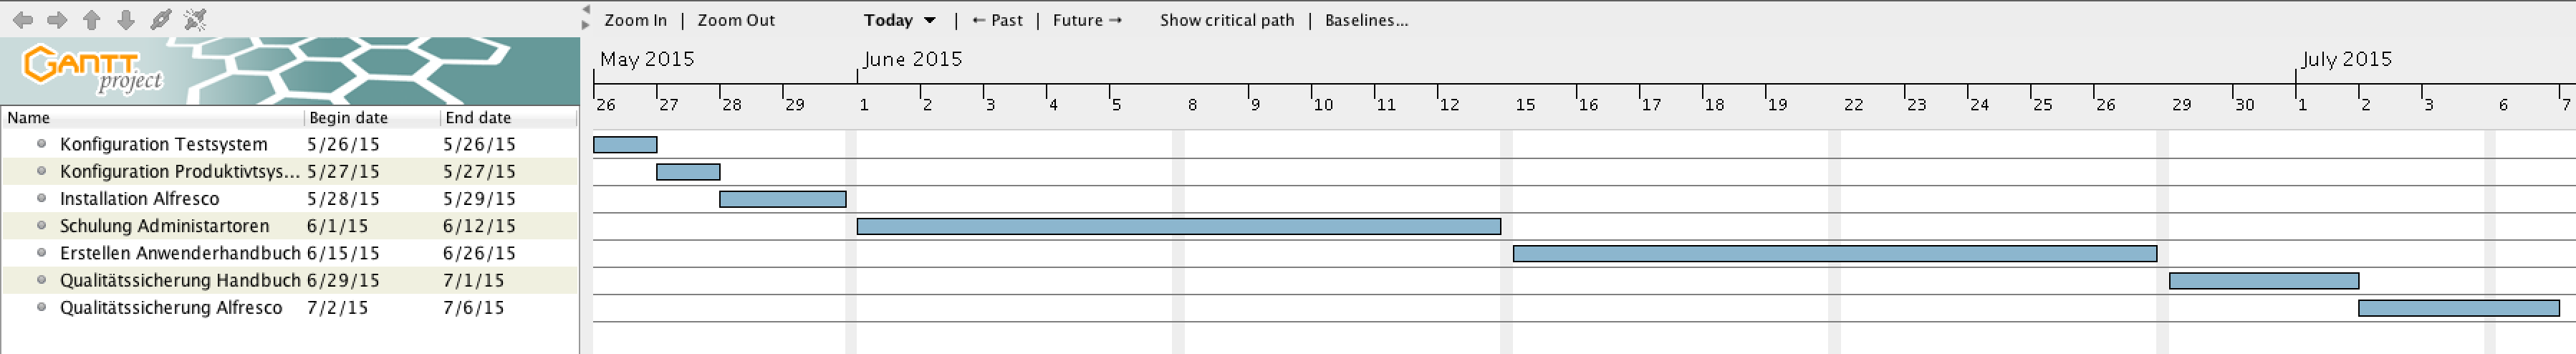
\includegraphics[width=\textwidth]
	{kapitel/gruppe4_2/bilder/gantt_diagramm_alfresco}
	\caption{Gantt Diagramm Alfresco}
	\label{fig_gantt_diagramm_alfresco}
\end{figure}

Das Gantt-Diagramm in Abbildung \ref{fig_gantt_diagramm_alfresco} zeigt die Dauer der einzelnen Teilschritte der Einführung des Teilprojektes „Alfresco“. Die Gesamtdauer des Teilprojekts ist die Strecke zwischen dem Anfang des obersten und dem Ende des untersten Balkens. Die Datumsangaben sind hier zu ignorieren, es geht nur um die Gesamtzahl an Manntagen, die die Umsetzung des Teilprojekts benötigt. Im ersten Schritt müssen die Server sowohl für Test- als auch für die Produktivsysteme konfiguriert und in das vorhandene Netzwerk integriert werden. Danach wird die Software installiert und entsprechend den Vorgaben der Fachbereiche konfiguriert. Nach der Installation können die Administratoren des DMS geschult werden um in dem nächsten Schritt ein Handbuch erstellen zu können. Die Qualitätsicherung des Handbuches und des DMS folgt zum Abschluss des Projekts. Ingesamt dauert die Einführung 30 MT.

\subsubsection{Redesign / Relaunch Hochschule-Webseite}
\label{subsubsection_redesign_webseite}
Um den Aufwand - und damit auch den Kosten- und Zeitrahmen der Umsetzung einer neuen Hochschulwebsite zu ermitteln, wurden Gespräche mit mehreren Experten\footnote{Achim Gosse, Geschäftsführender Gesellschafter digitalnoise GmbH (\url{www.digitalnoise.de})}\footnote{Stefan Becker, Software- und Webentwickler (\url{www.beckeste.de})} geführt.

Die Ergebnisse dieser Gespräche finden sich zusammengefasst in Tabelle \ref{tab_aufwand_redesign}, welche die verschiedenen Phasen des Entwicklungsprozesses, vom initialen Workshop bis hin zur Auslieferung und Qualitätsicherung, abbildet. Als Einheit wird dabei auf “Manntage” (MT) statt auf monetäre Angaben gesetzt, da Stunden- und Tagessätze teils starken regionalen Unterschieden unterliegen. Es gilt zu beachten, dass die hier durchgeführte Betrachtung der Kosten lediglich die externen Kosten berücksichtigt. Ausfallzeiten von Mitarbeitern, die beispielsweise durch die Teilnahme an Workshops generiert werden, werden nicht berücksichtigt.

\begin{table}
	\centering
	\begin{tabularx}{10cm}{@{}l *1{>{\raggedleft\arraybackslash}X}@{}}
		\hline \textbf{Aufgabe} & \textbf{Manntage} \\
			Workshop & 5\\
			Konzept & 10\\
			Präsentation Konzept & 2\\
			User experience & 5\\
			Design & 15\\
			Präsentation Design & 2\\
			Endpräsentation & 3\\
			technische Umsetzung & 2\\
			Anpassung Content & 5\\
			Qualitätssicherung & 3\\
			Deployment & 1\\
			Puffer & 5\\
			\textbf{Gesamt} & \textbf{48 - 53}\\
			
		\hline
	\end{tabularx}
	\caption{Aufwandsschätzung zum Redesign der Hochschule-Webseite}
	\label{tab_aufwand_redesign}
\end{table}

Der Initiale Schritt des gesamten Prozesses sollte, sofern im Voraus kein ausgearbeitetes Konzept vorliegt, in der Durchführung von Workshops mit Entscheidungsträgern aus allen beteiligten Bereichen (Verwaltung, Fachbereiche, Rechenzentrum, etc.) liegen. Um das Ziel des Workshops, nämlich eine gemeinsame Grundlage zu schaffen, die von allen gleichermaßen getragen wird, zu erreichen, werden, bedingt durch das vorhandene Konfliktpotential, 5 Manntage zur Durchführung angesetzt.

Die Ergebnisse des Workshops werden anschließend durch Konzeptioner, die an dem Workshop als “Zuhörer” teilgenommen haben, verarbeitet, um daraus ein Website-Konzept zu entwickeln. Für die Ausarbeitung des Konzepts mit entsprechender Präsen-tation vor den Projektverantwortlichen der Hochschule werden 12 Manntage veranschlagt.

Nachdem das Konzept freigegeben wurde, können User-Experience-Experten und (User Interface-)Designer mit der Ausarbeitung der Gestaltungsvorlage beginnen. Dabei ist es üblich, dem Kunden mehrere, möglichst unterschiedliche, Designvorschläge zu unterbreiten. Inklusive Präsentation und Ausarbeitung des finalen Vorschlags kann dieser Posten mit 22 Manntagen berechnet werden.

Auf Basis des verabschiedeten Designs kann die technische Realisierung der neuen Konzepte und Gestaltungsvorlagen beginnen. Da zum einen die benötigten Kompetenzen innerhalb der Hochschule vorhanden sind und zum anderen das interne Konfliktpotential in diesem Schritt wesentlich geringer ausfällt, bietet es sich an, diesen Schritt hochschulintern durchzuführen. Die kalkulierten 7 Manntage durch die Dienstleister setzen sich aus den Punkten “technische Umsetzung” (2 Manntage) und “Anpassung Content” (5 Manntage) zusammen. Die 2 Mantage der techniscnhe Umsetzung sind dabei zur Unterstützung des Hochschulteams vorgesehen, während die 5 Tage vor allem genutzt werden, um auf “content-seitige” Sonderfälle reagieren zu können. Da bereits TYPO3 als Content Management System zum Einsatz kommt, sollte die Migration des bestehenden Inhalts in ein neues System entfallen. Durch die Möglichkeit des Multi-Channel-Publishings und Hilfsmittel zur Erstellung barrierearmer Websites ist ein Wechsel des Systems nicht erforderlich.

Vor der Auslieferung und dem “live gehen” des Internetauftritts steht noch die finale Qualitätssicherung. Dabei wird die gesamte Webpräsenz abschließend auf Konsistenz und Fehlerfreiheit geprüft. Bei einer Website diesen Umfangs werden für die Überprüfung und Korektur eventueller Fehler 3 Manntage berechnet.

Die eigentliche Auslieferung sollte nach der Qualitätssicherung innerhalb eines Arbeitstages durchgeführt sein. Zur Absicherung wird eine Arbeitswoche als Puffer veranschlagt, sodass die Umsetzung des Projekts im Kostenrahmen von 48 bis 53 Manntagen liegt.

Da das Erstellen eines Konzepts für einen komplexen Internetauftritt im Allgemeinen mit einem nicht zu unterschätzenden Aufwand verbunden ist, wird ein solches Konzept durch die entsprechenden Agenturen in der Regel nur angefertigt, wenn dahinter die Aussicht auf den Erhalt des entsprechenden Auftrags steht. Da weder ein bestehendes Konzept, noch die konkrete Aussicht auf einen tatsächlichen Auftrag vorliegen, konnten durch die Dienstleister keine konkreten Angebote abgegeben werden.

\subsubsection{Facebook Seite}
Facebook unterscheidet verschiedene Arten von Applikationen die mit einem Profil verknüpft werden können. Dabei ist es unerheblich ob dieses Profil einer Privatperson, einem Unternehmen oder einer anderen Organisation zugeordnet wird.\footnote{\url{https://developers.facebook.com/docs}}

Die Hochschule Emden/Leer hat bereits ein reguläres Facebook Profil. Es gilt nun für die einzelnen Fachbereiche sogenannte “Page Tabs” einzurichten. “Page Tabs” werden auf einer Facebook Profil-Seite als Menü-Links eingeblendet. Der Inhalt der Tabs wird wird mit einer, nach speziellen Vorgaben gestalteten, Webseite in die Profil-Seite integriert. Facebook gibt mit einer API das Format vor. Auch die Nutzung anderer Elemente der Facebook Dienste bedarf einer Integration der Facebook API. Dabei ist zu beachten, dass die Webseite, deren Inhalt in dem Tab angezeigt wird, auf einem externen Server, in diesem Fall einem Server der Hochschule, liegt.\footnote{\url{https://developers.facebook.com/docs}}

Bei der Ermittlung des Zeitbedarfs für die Erstellung eines Tabs geht es folglich darum, den zeitlichen Aufwand für das Anfertigen einer regulären Webseite nach den Vorgaben der Facebook API zu schätzen. 

Die benötigten Funktionen einer solchen Webseite und der dazugehörige Entwicklungsaufwand werden wieder durch Befragung eines Experten ermittelt. Als Experte für dieses Teilprojekt stand Herr Dipl.-Inf. Franz Riehl von der jambit GmbH aus München zur Verfügung. Analog zur Kalkulation der Website in Kapitel \ref{subsubsection_redesign_webseite} wird auch in diesem Fall in “Manntagen” gerechnet:

\begin{table}
	\centering
	\begin{tabularx}{10cm}{@{}l *1{>{\raggedleft\arraybackslash}X}@{}}
		\hline \textbf{Aufgabe} & \textbf{Manntage} \\
		Konzept & 1\\
		Design & 10\\
		Präsentation & 1\\
		Realisierung & 8\\
		Integration & 1\\
		Abnahme / QS & 1\\
		\textbf{Gesamt} & \textbf{22}\\
		
		\hline
	\end{tabularx}
	\caption{Aufwandsschätzung zur Entwicklung der "Facebook Page Tabs"}
	\label{tab_aufwand_facebook_page}
\end{table}

Der initiale Schritt besteht erneut in der Konzeption der einzubindenden Webanwendung. Da das Konzept der Page-Tabs für jeden Fachbereich identisch sein sollte, fällt der konzeptionelle Aufwand nur einmalig an. Das Konzept besteht in diesem Fall aus der Auswahl der zu transportierenden Informationen und einer entsprechenden Darstellungsform, wofür 1 Manntag kalkuliert wird.

Im Gegensatz zum Konzept sollte die Gestaltung der Page-Tabs an den jeweiligen Fachbereich angepasst werden. Da es im Idealfall bereits ein Corporate-Design Manual gibt, in dem grundlegende Gestaltungsrichtlinien festgehalten sind, werden für diesen Schritt 2,5 Tage pro Fachbereich berechnet, sodass in Summe 10 Manntage berücksichtigt werden müssen.

Nach der Präsentation aller vier Designs, wofür 1 Manntag veranschlagt wird, folgt die Realisierung. Da die Gestaltung an die Fachbereiche angepasst wurde, können die Vorlagen voraussichtlich nicht alle nach dem gleichen Schema umgesetzt werden, weshalb für jeden Page-Tab 2 Manntage kalkuliert werden.

Die finalen Schritte bestehen in der Facebook-Integration mit abschließender Qualitäts-sicherung. Pro Fachbereich kann diesbezüglich ein halber Manntag vorgesehen werden, sodass die letzten Punkte mit insgesamt 2 Manntagen zu Buche schlagen. Die Gesamtsumme beträgt bei dem beschriebenen Vorgehen 22 Manntage.

Da es sich bei dem Facebook-Auftritt nicht um ein “kritisches System” im Sinne der Verfügbarkeit der Anwendung handelt, bietet es sich an, die Webanwendungen im Rahmen einer Projekt- oder Bachelorarbeit umsetzen zu lassen. Neben der Tatsache, dass so die Gestaltung und Umsetzung “direkt durch die Zielgruppe” des Auftritts geschieht, können dadurch Kosten eingespart werden. Alternativ sollte auf studentische Hilfskräfte zurückgegriffen werden.

Eine exemplarische Kalkulation auf Grundlage der bereits in Kapitel \ref{subsubsection_dokusystem_alfresco} erfassten Stundensätze zeigt Tabelle \ref{tab_kosten_umsetzung_facebook}.

\begin{table}[h!]
	\centering
	\begin{tabularx}{\textwidth}{l|r|l|*1{>{\raggedleft\arraybackslash}X}@{}}
		\hline \textbf{Aufgabe} & \textbf{Manntage} & \textbf{Personalkostenkategorie} & \textbf{Betrag} \\
		Konzept & 1 & studentische Hilfskraft & 13,65\\
		Design & 10 & studentische Hilfskraft & 136,50\\
		Präsentation & 0,5 & studentische Hilfskraft & 6,83\\
		 & 0,5 & Nichtwissenschaftlicher MItarbeiter & 12,90\\
		Realisierung & 8 & studentische Hilfskraft & 109,20\\
		Integration & 1 & studentische Hilfskraft & 13,65\\
		Abnahme / QS & 1 & Nichtwissenschaftlicher MItarbeiter & 25,80\\
		\textbf{Gesamt} & \textbf{21,5} & & \textbf{318,53}\\
		
		\hline
	\end{tabularx}
	\caption{Exemplarische Kostenkalkulation der Umsetzung der "Facebook Page Tabs"}
	\label{tab_kosten_umsetzung_facebook}
\end{table}

Die Realisierung der Page-Tabs durch eine studentische Hilfskraft würde folglich ca. 350 Euro kosten. Da die Präsentation vermutlich vor einem nichtwissenschaftlichen Mitarbeiter gehalten wird, müssen auch dessen Personalkosten für den Zeitraum der Präsentation berücksichtigt werden. Ebenso erfolgt die Abnahme und Qualitätssicherung voraussichtlich durch einen nichtwissenschaftlichen Mitarbeiter.